\section{ownCloud konfigurieren}
Hat man ownCloud erfolgreich installiert, muss die Grundkonfiguration vorgenommen werden. Auf die installierte Cloud kann über den Webbrowser zugegriffen werden. Dazu muss man lediglich die IP-Adresse, die man während der Installation durch den Befehl \textit{ifconfig} ermittelt hat, in die Adresszeile des Browsers eingegeben werden. Das würde dann - abgesehen von den letzten zwei Ziffern - in etwa so aussehen:

\begin{lstlisting}
http://192.168.1.107
\end{lstlisting}

\subsection{Administrator-Account anlegen}
Kann der Browser sich mit der Cloud verbinden, wird die Startseite angezeigt. ownCloud verlangt vom Benutzer bei erstmaligem Aufruf, einen Administrator-Account anzulegen. Der Administrator verwaltet die Cloud, kann wichtige Einstellungen vornehmen und Benutzer anlegen.
\\
\\
Um einen Administrator-Account anzulegen, muss man lediglich den gewünschten Benutzernamen und ein Passwort definieren. Es empfiehlt sich hier einen guten, aussagekräftigen Namen zu wählen, den man sich gut merken kann. Das Passwort soll vor allen Dingen sicher sein. Natürlich ist es nur von Vorteil, wenn man es sich auch leicht merken kann.
\\
\\
Bevor der Account mittels Klick auf \textit{Finish Setup} erstellt wird, sollte man noch festlegen, welches das Basisverzeichnis für alle in der Cloud gespeicherten Daten ist. Man sollte hier den Pfad eingeben, unter dem das Speichergerät eingebunden wurde. In diesem Fall also:

\begin{lstlisting}
\mnt\ownclouddata
\end{lstlisting}

\begin{figure}[h]
\centering
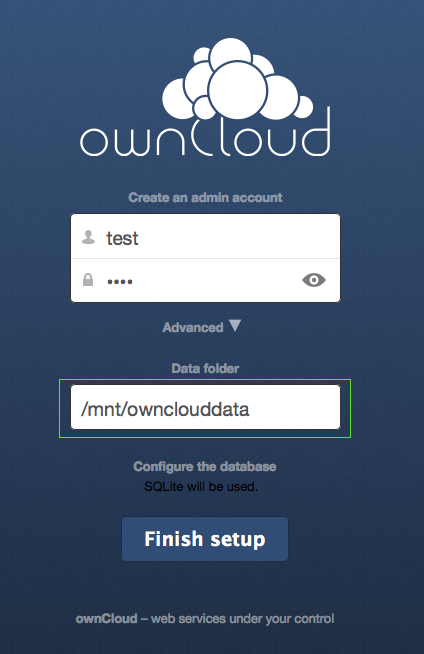
\includegraphics[scale=0.5]{images/admin_setup}
\caption{Administrator-Account anlegen}
\end{figure}

\subsection{Webinterface}
Nach erfolgreicher Erstellung des Administrator-Accounts wird man auf das Webinterface der Cloud weitergeleitet. Es begrüsst einem zuerst ein \textit{Welcome Screen}. Er liefert nützliche Informationen und Links zu Dokumentationen und Programmen, die mit ownCloud zusammen genutzt werden können.

\begin{figure}[h]
\centering
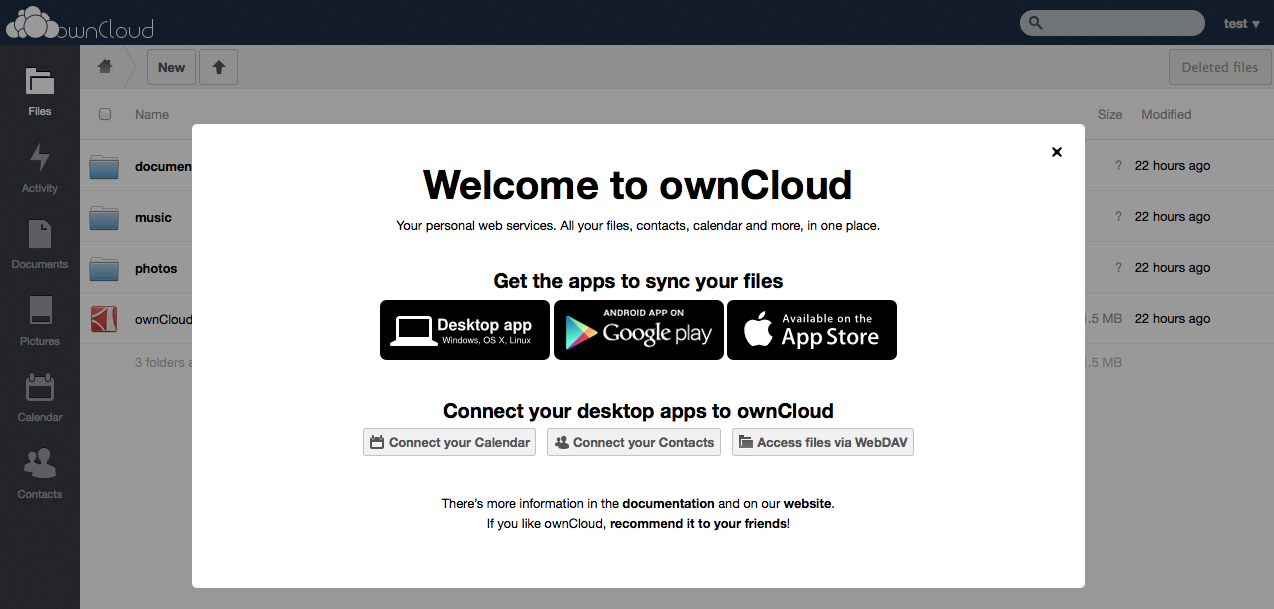
\includegraphics[scale=0.4]{images/welcomescreen}
\caption{Welcome Screen}
\end{figure}

Es gibt für ownCloud ein Client-Programm, welches auf Windows, OS X und Linux verfügbar ist. Es ist eine Alternative zum Webinterface und ermöglicht es, Dateien auf dem Computer mit der Cloud zu synchronisieren. Die Köpfe hinter ownCloud haben ebenfalls eine App für das Smartphone kreiert und stellen diese auf dem Google Play (Android) und dem AppStore (iOS) zur Verfügung. Auf diese Anwendungen an dieser Stelle im Detail einzugehen, würde aber den Rahmen dieser Arbeit sprengen. Es gibt zudem viele gute Dokumentation im Netz, die bei Problemen herangezogen werden können. Im Normalfall werden diese aber wohl kaum benötigt, da sehr vieles selbsterklärend und einfach von der Hand geht.

Folgender Link führt zur offiziellen Webseite, von der der Client heruntergeladen werden kann: \url{http://owncloud.org/sync-clients/}

\subsection{Sicherheitseinstellungen vornehmen}
Bevor ownCloud produktiv genutzt wird, sollte man als Administrator noch gewisse Sicherheitseinstellungen vornehmen. Dazu klickt man auf das Menü am rechten oberen Bildschirm rand und wählt \textit{Admin}.

\begin{figure}[h]
\centering
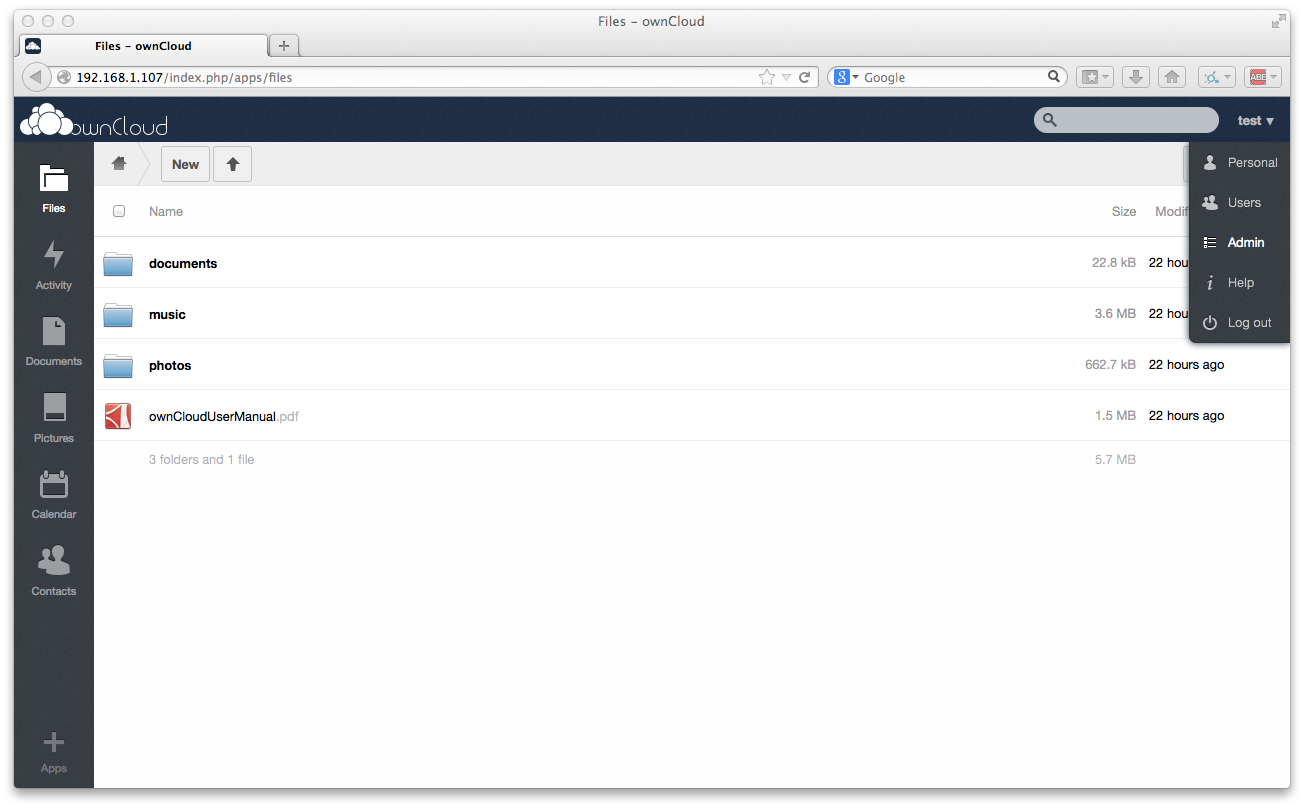
\includegraphics[scale=0.5]{images/admin_settings}
\caption{Administrator-Einstellungen}
\end{figure}

ownCloud bemerkt, wenn man sich mittels HTTP anmeldet, denn bei Verwendung von HTTP ist die Verbindung nicht verschlüsselt. Es wird deshalb als Erstes eine Warnmeldung angezeigt, die einem auf das bestehende Risiko aufmerksam macht.

\begin{figure}[h]
\centering
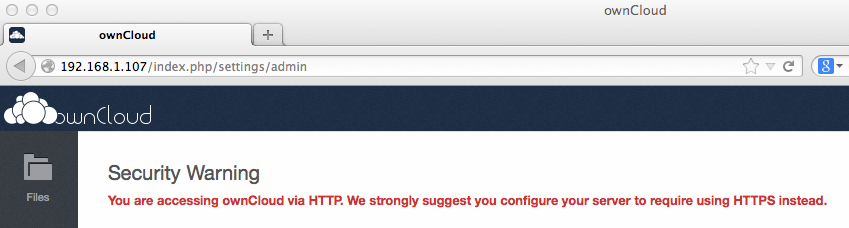
\includegraphics[scale=0.6]{images/security_warning}
\caption{Sicherheitswarnung}
\end{figure}

Um eine sichere Verbindung zu ownCloud herzustellen, könnte man jedes Mal die Adresszeile dementsprechend anpassen:

\begin{lstlisting}
https://192.168.1.107
\end{lstlisting}

Dies kann aber leicht vergessen werden und ist zudem aufwendig. ownCloud ermöglicht es glücklicherweise, die Verwendung von HTTPS automatisch zu erzwingen. Dazu muss man lediglich zum Bereich \textit{Security} gehen. Wird das Kästchen mit dem Titel \textit{Enforce HTTPS} aktiviert, baut ownCloud mit jedem Benutzer automatisch eine sichere Verbindung auf.

\begin{figure}[h]
\centering
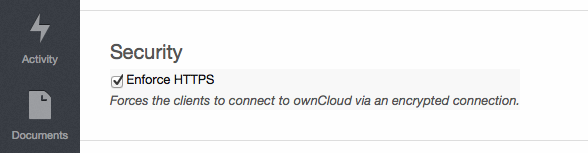
\includegraphics[scale=0.5]{images/https_checkbox_ticked}
\caption{HTTPS aktivieren}
\end{figure}

Es muss dazu noch gesagt werden, dass diese Einstellung lediglich vorgenommen werden kann, wenn man schon per HTTPS mit der Cloud verbunden ist.
\\
\\
Fürs Erste wär's das auch schon. Jeder Benutzer, der sich von nun an mit der Cloud verbindet, baut automatisch eine sichere, verschlüsselte Verbindung auf. Dies erkennt man an dem \textit{https://} in der Adresszeile und je nach verwendetem Webbrowser an dem kleinen Schloss-Symbol davor.

\begin{figure}[h]
\centering
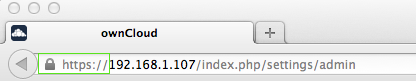
\includegraphics[scale=0.65]{images/https_connection}
\caption{HTTPS aktiviert}
\end{figure}

\subsection{Abschluss}
Die Basiskonfiguration von ownCloud ist fertig. Jetzt ist es an der Zeit, sich mit den sonstigen Funktionalitäten und Einstellungen der Anwendung vertraut zu machen. Es gibt dazu wie immer eine grosse Zahl an Hilfestellungen im Netz.
Folgende sollen als erste Anlaufstelle dienen:

\begin{itemize}
\item Administrator-Anleitung, Englisch: \url{http://doc.owncloud.org/server/6.0/admin_manual/}
\item Benutzer-Anleitung, Englisch \url{http://doc.owncloud.org/server/6.0/user_manual/}
\item Client-Anleitung, Englisch \url{http://doc.owncloud.org/desktop/1.5/}
\end{itemize}
